
\title{T-61.5130 Machine Learning and Neural Networks}
\author{Karhunen, Luttinen}
\date{Exercise 7, ??.??.2012}

\newcommand{\vect}[1]{{\bf{#1}}}
\newcommand{\svect}[1]{\boldsymbol{#1}}
\newcommand{\matr}[1]{\boldsymbol{#1}}


\begin{document}

\maketitle

\begin{enumerate}

\item Consider on a general level the major differences (and similarities)
  between radial-basis function (RBF) networks and multilayer perceptron
  (MLP) networks.

  \begin{solution}

    \begin{itemize}
    \item Both RBF and MLP networks are nonlinear layered networks having
      universal approximation properties (that is, they are able to
      approximate any smooth enough function to an arbitrary degree of accuracy).
    \item The most important differences between them are:
      % 
      \begin{enumerate}
      \item An RBF network has a single hidden layer, while an MLP can have
        several hidden layers.
      \item The computational nodes in the MLP network are similar in various layers,
        while in the RBF network they are quite different in the output
        and hidden layers.
      \item In the RBF network, the output layer is linear, while it is usually
        nonlinear in an MLP network.
      \item In each hidden node, the activation function of RBF network computes
        an {\em Euclidean distance}, while in MLP networks an {\em inner product}
        between the input and the weight vector is computed.
      \item MLPs construct {\em global} approximations, while RBF networks
        approximate {\em locally} nonlinear input-output mappings.
      \end{enumerate}
      % 
    \item MLP may require less parameters than the RBF network for achieving
      the same accuracy.
    \end{itemize}

  \end{solution}
  

\item The well-known XOR (Exclusive OR) problem is the simplest example of a
  two-class classification problem where the pattern vectors are not linearly
  separable. In the XOR problem, there are four two-dimensional input vectors
  (patterns) (0,0), (0,1), (1,1), and (1,0). The first and third pattern
  vector belong to the class 1, while the second and the fourth one belong
  to the class 2. Solve the XOR problem by using a RBF network with two
  Gaussian basis functions centered at ${\bf c}_1 = (0,1)^T$ and
  ${\bf c}_2 = (1,0)^T$.

  \begin{solution}

    RBF network for solving the XOR problem

    \begin{center}
      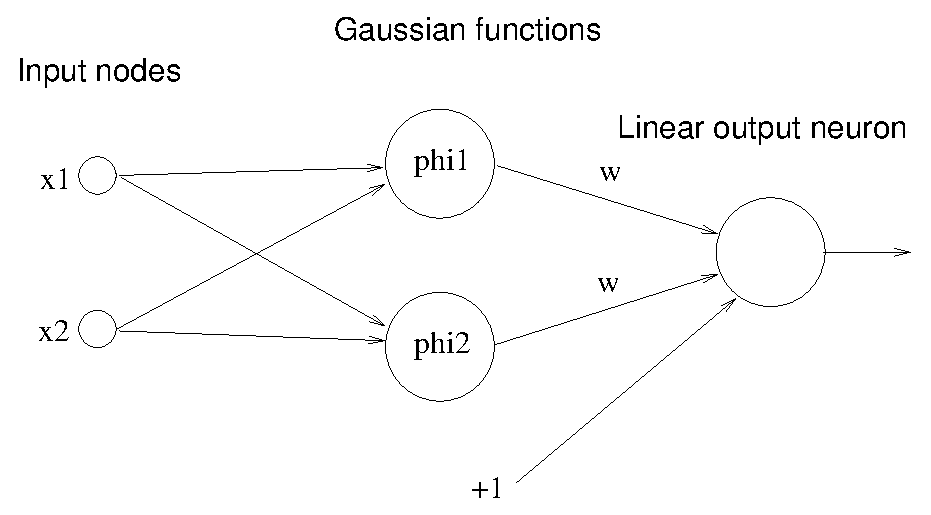
\includegraphics[scale=0.7]{v102-f1.eps}
    \end{center}

    Some notes on the above network:
    \begin{itemize}
    \item weight sharing is justified by the symmetry of the problem
    \item the desired output values of the problem have nonzero mean and
      thus the output unit includes a bias 
    \end{itemize}
    Now the centers of the radial-basis functions are
    \begin{eqnarray*}
      \mathbf{t}_1&=&(-1,1)^T\\
      \mathbf{t}_2&=&(1,-1)^T.
    \end{eqnarray*}

    Let us assume that the logical symbol 0 is represented by level -1
    and symbol 1 is represented by level +1. Sometimes this is directly
    taken as the XOR problem.

    \begin{enumerate}
    \item For the input pattern (0,0):\\
      $\mathbf{x}=(-1,-1)^T$ and
      \begin{eqnarray*}
        (1)\;G(\|\mathbf{x}-\mathbf{t}_1\|)&=&e^{-\|(-1,-1)^T-(-1,1)^T\|^2}\\
        &=&e^{-\|(0,-2)^T\|^2}=e^{-4}=0.01832\\
        (2)\;G(\|\mathbf{x}-\mathbf{t}_2\|)&=&e^{-\|(-1,-1)^T-(1,-1)^T\|^2}\\
        &=&e^{-\|(-2,0)^T\|^2}=e^{-4}=0.01832
      \end{eqnarray*}

    \item For the input pattern (0,1):\\
      $\mathbf{x}=(-1,1)^T$ and
      \begin{eqnarray*}
        (3)\;G(\|\mathbf{x}-\mathbf{t}_1\|)&=&e^{-\|(-1,1)^T-(-1,1)^T\|^2}\\
        &=&e^{-\|(0,0)^T\|^2}=e^{-0}=1\\
        (4)\;G(\|\mathbf{x}-\mathbf{t}_2\|)&=&e^{-\|(-1,1)^T-(1,-1)^T\|^2}\\
        &=&e^{-\|(-2,2)^T\|^2}=e^{-8}=0.000336
      \end{eqnarray*}

    \item For the input pattern (1,1):\\
      $\mathbf{x}=(1,1)^T$ and
      \begin{eqnarray*}
        (5)\;G(\|\mathbf{x}-\mathbf{t}_1\|)&=&e^{-\|(1,1)^T-(-1,1)^T\|^2}\\
        &=&e^{-\|(2,0)^T\|^2}=e^{-4}=0.01832\\
        (6)\;G(\|\mathbf{x}-\mathbf{t}_2\|)&=&e^{-\|(1,1)^T-(1,-1)^T\|^2}\\
        &=&e^{-\|(0,2)^T\|^2}=e^{-4}=0.01832
      \end{eqnarray*}

    \item For the input pattern (1,0):\\
      $\mathbf{x}=(1,-1)^T$ and
      \begin{eqnarray*}
        (7)\;G(\|\mathbf{x}-\mathbf{t}_1\|)&=&e^{-\|(1,-1)^T-(-1,1)^T\|^2}\\
        &=&e^{-\|(2,-2)^T\|^2}=e^{-8}=0.000336\\
        (8)\;G(\|\mathbf{x}-\mathbf{t}_2\|)&=&e^{-\|(1,-1)^T-(1,-1)^T\|^2}\\
        &=&e^{-\|(-0,0)^T\|^2}=e^{-0}=1
      \end{eqnarray*}
    \end{enumerate}

    Results (1)-(8) are combinded as a matrix
    \begin{equation*}
      \mathbf{G}=\begin{array}{cl}
        \begin{array}{ccc}
          \varphi_1(\mathbf{x})&\varphi_2(\mathbf{x})&\mbox{bias}
        \end{array} &\\
        \left[
          \begin{array}{ccc}
            e^{-4} & e^{-4} & 1\\
            1 & e^{-8}& 1\\
            e^{-4} & e^{-4} & 1\\
            e^{-8}& 1 & 1
          \end{array}
        \right] &
        \begin{array}{r}
          \mbox{ pattern }(0,0)\\
          (0,1)\\
          (1,1)\\
          (1,0)
        \end{array}
      \end{array}
    \end{equation*}
    and the desired responses as vector $d=(-1,1,-1,1)^T$.

    The linear parameters of the network are defined by
    \begin{equation*}
      \mathbf{Gw}=\mathbf{d}\mbox{, where }\mathbf{w}=(w,\;w,\;b)^T.
    \end{equation*}

    The solution to the equation is
    $\mathbf{w}=\mathbf{G}^\dagger\mathbf{d}$, where $\mathbf{G}^\dagger=(\mathbf{G}^T\mathbf{G})^{-1}\mathbf{G}^T$
    is the pseudo inverse of $\mathbf{G}$

    \begin{equation*}
      \mathbf{G}^\dagger=
      \left[
        \begin{array}{rrrr}
          -0.5188 & 1.0190 & -0.5188 &0.0187\\
          -0.5188 & 0.0187 & -0.5188 &1.0190\\
          -0.5190 & -0.0190 & -0.5190 &-0.0190
        \end{array}\right]
    \end{equation*}
    \begin{equation*}
      \mathbf{w}=(2.0753,\;2.0753,\;-1.076)^T
    \end{equation*}


  \end{solution}
  
\item Derive the learning rules for the stochastic gradient method for
  training an RBF neural network.

  \begin{solution}

  \end{solution}
  
  
\item Consider approximation of the nonlinear function $y = e^{-x} \sin(3x)$
  on the interval $[0,4]$ using multilayer perceptron (MLP) and radial-basis
  function (RBF) networks. Compare the generalization ability of these
  networks.

  \begin{solution}

    See Ham \& Kostanic examples 3.2 and 3.4.
  \end{solution}

  
\item In Ham's and Kostanic's book, training of RBF networks is considered for the
  case of a single neuron in the output layer only. Show how the learning method
  presented in section 3.6.1 can be generalized for several neurons in the
  output layer.

  \begin{solution}

    The learning method can be extended to networks with multiple neurons
    in the output layer by transforming the scalar equations (Ham \&
    Kostanic, Equations 3.147--3.154) into vector notation.

    In Eq. (3.147) the index $i$ is present in the weight vector $w_{ik}$
    denoting the $i$th output neuron and the $k$th hidden neuron, but in
    (3.148) the index has been dropped. Simply add the index $i$ for
    $\hat{y}(q)$ in (3.147) and indeces $i$ for $\hat{y}(q)$ and $w$ in
    (3.148), which then become $w_{i1}, w_{i2}$ etc.


    Then Eq. (3.149) for the $i$th neuron of the output layer is the same
    as in the book and in  $\hat{{\bf y}}$ ja ${\bf w}$ in $i$ is merely
    added to denote the neuron. The matrix $\Phi$ stays the same for all
    output neurons. An LMS solution can be obtained for each output
    neuron using (3.154), where an index $i$
    is added to denote the $i$th weight ${\bf w}_i$ and the
    $Q$-dimensional vector of its desired outputs ${\bf y}_{i,d}$.
    The obtained LMS solutions (3.154) can then be combined in matrix
    notation as
    \[
    \bf{W} = (\Phi^T \Phi)^{-1}\Phi^T \bf{Y}_d,\] 
    where the column vectors of the $N\times M$ weight matrix $\bf{W}$ are the output layer's $M$ neuron's
    weight vectors ${\bf w}_i$ and the column vectors ${\bf y}_{i,d}$ of the $Q \times M$ matrix $\bf{Y}_d$
    are the output layer's M neuron's desired output vectors for the
    set of $Q$ training samples.

  \end{solution}
  
\end{enumerate}
\end{document}             % End of document.

%%% Local Variables: 
%%% mode: latex
%%% TeX-master: "ex07_solutions"
%%% End: 
